\documentclass[tikz,border=2pt]{standalone}
\usepackage[T1]{fontenc}
\usepackage{mathpazo}
\usepackage{amsmath}
\usepackage{amssymb}
\usetikzlibrary{arrows.meta,calc,positioning}

\definecolor{ink}{HTML}{17202A}
\definecolor{navy}{HTML}{173A63}
\definecolor{teal}{HTML}{2F686B}
\definecolor{ochre}{HTML}{C96F00}
\definecolor{success}{HTML}{2F6B36}
\definecolor{openred}{HTML}{A72F22}
\definecolor{muted}{HTML}{65717C}
\definecolor{rulegray}{HTML}{AEB6BF}

\tikzset{
  panel/.style={draw=navy, line width=.42pt, fill=white},
  fine/.style={draw=ink, line width=.38pt},
  faint/.style={draw=rulegray, line width=.32pt},
  dot/.style={circle, draw=ink, fill=white, line width=.35pt,
              inner sep=0pt, minimum size=2.5pt},
  check/.style={text=success, font=\bfseries\fontsize{6.5}{7}\selectfont},
  every node/.style={text=ink}
}

\newcommand{\bodyfont}{\fontsize{7.35}{8.8}\selectfont}
\newcommand{\smallfont}{\fontsize{6.35}{7.4}\selectfont}
\newcommand{\tinyfont}{\fontsize{5.5}{6.3}\selectfont}
\newcommand{\titlefont}{\bfseries\fontsize{10.0}{11}\selectfont}
\newcommand{\sectionfont}{\bfseries\fontsize{11.5}{12.5}\selectfont}
\newcommand{\resultfont}{\bfseries\fontsize{12}{13}\selectfont}

\newcommand{\panelbox}[4]{%
  \begin{scope}[shift={(#1,#2)}]
    \draw[panel] (0,0) rectangle (4.06,4.88);
    \node[anchor=west,font=\titlefont,text=#4] at (.24,4.56) {#3};
  \end{scope}%
}

\newcommand{\roles}[4]{%
  \node[anchor=north west,font=\bfseries\bodyfont,text=ochre] at (.24,#1) {PI};
  \node[anchor=north west,align=left,text width=2.45cm,font=\bodyfont]
    at (1.35,#1) {#2};
  \node[anchor=north west,font=\bfseries\bodyfont,text=navy] at (.24,#3) {Student};
  \node[anchor=north west,align=left,text width=2.45cm,font=\bodyfont]
    at (1.35,#3) {#4};
}

\begin{document}
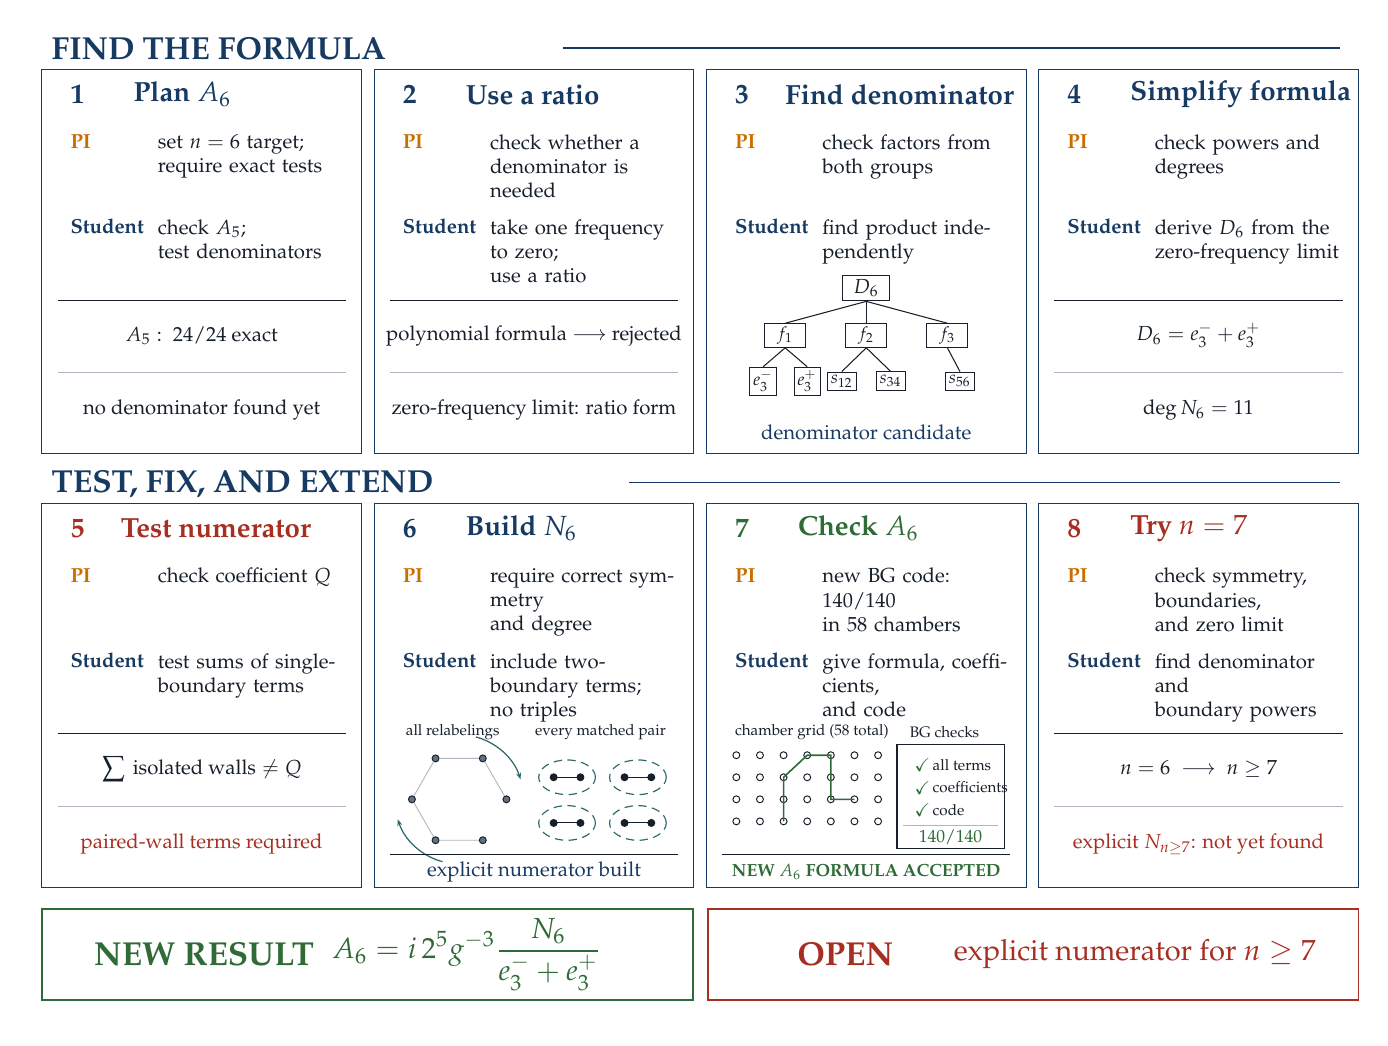
\begin{tikzpicture}[x=1cm,y=1cm]
  \fill[white] (-.02,-.02) rectangle (16.82,12.55);

  % Section 1 heading
  \node[anchor=west,font=\sectionfont,text=navy] at (.16,12.28)
    {FIND THE FORMULA};
  \draw[navy,line width=.48pt] (6.78,12.29)--(16.64,12.29);

  % Panel 1
  \begin{scope}[shift={(.16,7.14)}]
    \draw[panel] (0,0) rectangle (4.06,4.88);
    \node[anchor=west,font=\titlefont,text=navy] at (.24,4.56) {1};
    \node[anchor=west,font=\titlefont,text=navy] at (1.04,4.56) {Plan $A_6$};
    \roles{4.18}{set $n=6$ target;\newline require exact tests}
          {3.10}{check $A_5$;\newline test denominators}
    \draw[fine] (.20,1.95)--(3.86,1.95);
    \node[font=\bodyfont] at (2.03,1.50) {$A_5:\ 24/24\ \text{exact}$};
    \draw[faint] (.20,1.03)--(3.86,1.03);
    \node[font=\bodyfont] at (2.03,.55) {no denominator found yet};
  \end{scope}

  % Panel 2
  \begin{scope}[shift={(4.38,7.14)}]
    \draw[panel] (0,0) rectangle (4.06,4.88);
    \node[anchor=west,font=\titlefont,text=navy] at (.24,4.56) {2};
    \node[anchor=west,font=\titlefont,text=navy] at (1.04,4.56) {Use a ratio};
    \roles{4.18}{check whether a\newline denominator is needed}
          {3.10}{take one frequency to zero;\newline use a ratio}
    \draw[fine] (.20,1.95)--(3.86,1.95);
    \node[font=\bodyfont] at (2.03,1.50)
      {polynomial formula $\longrightarrow$ rejected};
    \draw[faint] (.20,1.03)--(3.86,1.03);
    \node[font=\bodyfont] at (2.03,.55)
      {zero-frequency limit: ratio form};
  \end{scope}

  % Panel 3: denominator structure (schematic 1 of 3)
  \begin{scope}[shift={(8.60,7.14)}]
    \draw[panel] (0,0) rectangle (4.06,4.88);
    \node[anchor=west,font=\titlefont,text=navy] at (.24,4.56) {3};
    \node[anchor=west,font=\titlefont,text=navy] at (.88,4.56) {Find denominator};
    \roles{4.18}{check factors from both groups}
          {3.10}{find product independently}

    \node[draw=ink,line width=.35pt,minimum width=.60cm,minimum height=.32cm,
          inner sep=1pt,font=\bodyfont] (D) at (2.03,2.10) {$D_6$};
    \node[draw=ink,line width=.35pt,minimum width=.52cm,minimum height=.30cm,
          inner sep=.5pt,font=\smallfont] (fone) at (1.00,1.50) {$f_1$};
    \node[draw=ink,line width=.35pt,minimum width=.52cm,minimum height=.30cm,
          inner sep=.5pt,font=\smallfont] (ftwo) at (2.03,1.50) {$f_2$};
    \node[draw=ink,line width=.35pt,minimum width=.52cm,minimum height=.30cm,
          inner sep=.5pt,font=\smallfont] (fthree) at (3.06,1.50) {$f_3$};
    \draw[fine] (D.south)--(fone.north);
    \draw[fine] (D.south)--(ftwo.north);
    \draw[fine] (D.south)--(fthree.north);
    \node[draw=ink,line width=.32pt,inner sep=1.2pt,font=\smallfont] (em) at (.72,.92) {$e_3^{-}$};
    \node[draw=ink,line width=.32pt,inner sep=1.2pt,font=\smallfont] (ep) at (1.28,.92) {$e_3^{+}$};
    \draw[fine] (fone.south)--(em.north);
    \draw[fine] (fone.south)--(ep.north);
    \node[draw=ink,line width=.32pt,inner sep=1.2pt,font=\smallfont] (s12) at (1.72,.92) {$s_{12}$};
    \node[draw=ink,line width=.32pt,inner sep=1.2pt,font=\smallfont] (s34) at (2.34,.92) {$s_{34}$};
    \draw[fine] (ftwo.south)--(s12.north);
    \draw[fine] (ftwo.south)--(s34.north);
    \node[draw=ink,line width=.32pt,inner sep=1.2pt,font=\smallfont] (s56) at (3.22,.92) {$s_{56}$};
    \draw[fine] (fthree.south)--(s56.north);
    \node[font=\bodyfont,text=navy] at (2.03,.27) {denominator candidate};
  \end{scope}

  % Panel 4
  \begin{scope}[shift={(12.82,7.14)}]
    \draw[panel] (0,0) rectangle (4.06,4.88);
    \node[anchor=west,font=\titlefont,text=navy] at (.24,4.56) {4};
    \node[anchor=west,font=\titlefont,text=navy] at (1.04,4.56) {Simplify formula};
    \roles{4.18}{check powers and\newline degrees}
          {3.10}{derive $D_6$ from the\newline zero-frequency limit}
    \draw[fine] (.20,1.95)--(3.86,1.95);
    \node[font=\bodyfont] at (2.03,1.50) {$D_6=e_3^-+e_3^+$};
    \draw[faint] (.20,1.03)--(3.86,1.03);
    \node[font=\bodyfont] at (2.03,.55) {$\deg N_6=11$};
  \end{scope}

  % Section 2 heading
  \node[anchor=west,font=\sectionfont,text=navy] at (.16,6.76)
    {TEST, FIX, AND EXTEND};
  \draw[navy,line width=.48pt] (7.62,6.77)--(16.64,6.77);

  % Panel 5
  \begin{scope}[shift={(.16,1.63)}]
    \draw[panel] (0,0) rectangle (4.06,4.88);
    \node[anchor=west,font=\titlefont,text=openred] at (.24,4.56) {5};
    \node[anchor=west,font=\titlefont,text=openred] at (.88,4.56) {Test numerator};
    \roles{4.18}{check coefficient $Q$}
          {3.10}{test sums of single-\newline boundary terms}
    \draw[fine] (.20,1.95)--(3.86,1.95);
    \node[font=\bodyfont] at (2.03,1.50)
      {$\displaystyle \sum \text{ isolated walls}\neq Q$};
    \draw[faint] (.20,1.03)--(3.86,1.03);
    \node[font=\bodyfont,text=openred] at (2.03,.55) {paired-wall terms required};
  \end{scope}

  % Panel 6: numerator assembly (schematic 2 of 3)
  \begin{scope}[shift={(4.38,1.63)}]
    \draw[panel] (0,0) rectangle (4.06,4.88);
    \node[anchor=west,font=\titlefont,text=navy] at (.24,4.56) {6};
    \node[anchor=west,font=\titlefont,text=navy] at (1.04,4.56) {Build $N_6$};
    \roles{4.18}{require correct symmetry\newline and degree}
          {3.10}{include two-boundary terms;\newline no triples}

    \node[anchor=west,font=\tinyfont] at (.28,1.97) {all relabelings};
    \foreach \a in {0,60,...,300}{
      \node[dot,fill=muted] (h\a) at ($(1.08,1.12)+(\a:0.60)$) {};
    }
    \draw[faint] (h0)--(h60)--(h120)--(h180)--(h240)--(h300)--cycle;
    \draw[-{Stealth[length=2.4pt]},teal,line width=.45pt]
      ($(1.08,1.12)+(75:.82)$) arc[start angle=75,end angle=18,radius=.82];
    \draw[-{Stealth[length=2.4pt]},teal,line width=.45pt]
      ($(1.08,1.12)+(255:.82)$) arc[start angle=255,end angle=198,radius=.82];

    \node[anchor=west,font=\tinyfont] at (1.92,1.97) {every matched pair};
    \foreach \yy in {1.40,.82}{
      \node[dot,fill=ink] at (2.28,\yy) {};
      \node[dot,fill=ink] at (2.62,\yy) {};
      \node[dot,fill=ink] at (3.18,\yy) {};
      \node[dot,fill=ink] at (3.52,\yy) {};
      \draw[fine] (2.28,\yy)--(2.62,\yy);
      \draw[fine] (3.18,\yy)--(3.52,\yy);
      \draw[teal,densely dashed,line width=.42pt]
        (2.45,\yy) ellipse[x radius=.36,y radius=.22];
      \draw[teal,densely dashed,line width=.42pt]
        (3.35,\yy) ellipse[x radius=.36,y radius=.22];
    }
    \draw[fine] (.20,.42)--(3.86,.42);
    \node[font=\bodyfont,text=navy] at (2.03,.20) {explicit numerator built};
  \end{scope}

  % Panel 7: verification (schematic 3 of 3)
  \begin{scope}[shift={(8.60,1.63)}]
    \draw[panel] (0,0) rectangle (4.06,4.88);
    \node[anchor=west,font=\titlefont,text=success] at (.24,4.56) {7};
    \node[anchor=west,font=\titlefont,text=success] at (1.04,4.56) {Check $A_6$};
    \roles{4.18}{new BG code: 140/140\newline in 58 chambers}
          {3.10}{give formula, coefficients,\newline and code}

    \node[anchor=west,font=\tinyfont] at (.24,1.98) {chamber grid (58 total)};
    \foreach \i in {0,...,6}{
      \foreach \j in {0,...,3}{
        \node[dot] at (.38+.30*\i,1.68-.28*\j) {};
      }
    }
    \draw[success,line width=.58pt]
      (.98,.84)--(.98,1.40)--(1.28,1.68)--(1.58,1.68)--(1.58,1.12)--(1.88,1.12);
    \node[anchor=west,font=\tinyfont] at (2.46,1.98) {BG checks};
    \draw[fine] (2.42,.50) rectangle (3.78,1.82);
    \node[check,anchor=west] at (2.52,1.56) {$\checkmark$};
    \node[anchor=west,font=\tinyfont] at (2.75,1.56) {all terms};
    \node[check,anchor=west] at (2.52,1.27) {$\checkmark$};
    \node[anchor=west,font=\tinyfont] at (2.75,1.27) {coefficients};
    \node[check,anchor=west] at (2.52,.98) {$\checkmark$};
    \node[anchor=west,font=\tinyfont] at (2.75,.98) {code};
    \draw[faint] (2.50,.79)--(3.70,.79);
    \node[font=\smallfont,text=success] at (3.10,.64) {140/140};
    \draw[fine] (.20,.42)--(3.86,.42);
    \node[align=center,font=\bfseries\smallfont,text=success] at (2.03,.20)
      {NEW $A_6$ FORMULA ACCEPTED};
  \end{scope}

  % Panel 8
  \begin{scope}[shift={(12.82,1.63)}]
    \draw[panel] (0,0) rectangle (4.06,4.88);
    \node[anchor=west,font=\titlefont,text=openred] at (.24,4.56) {8};
    \node[anchor=west,font=\titlefont,text=openred] at (1.04,4.56) {Try $n=7$};
    \roles{4.18}{check symmetry, boundaries,\newline and zero limit}
          {3.10}{find denominator and\newline boundary powers}
    \draw[fine] (.20,1.95)--(3.86,1.95);
    \node[font=\bodyfont] at (2.03,1.50) {$n=6\ \longrightarrow\ n\geq 7$};
    \draw[faint] (.20,1.03)--(3.86,1.03);
    \node[font=\bodyfont,text=openred] at (2.03,.55)
      {explicit $N_{n\geq 7}$: not yet found};
  \end{scope}

  % Final result bars
  \draw[success,line width=.62pt] (.16,.20) rectangle (8.43,1.36);
  \node[anchor=west,font=\resultfont,text=success] at (.70,.78) {NEW RESULT};
  \node[anchor=west,font=\fontsize{10.5}{12}\selectfont,text=success] at (3.72,.78)
    {$\displaystyle A_6=i\,2^5g^{-3}\frac{N_6}{e_3^-+e_3^+}$};

  \draw[openred,line width=.62pt] (8.62,.20) rectangle (16.88,1.36);
  \node[anchor=west,font=\resultfont,text=openred] at (9.63,.78) {OPEN};
  \node[anchor=west,font=\fontsize{10.5}{12}\selectfont,text=openred] at (11.62,.78)
    {explicit numerator for $n\geq 7$};
\end{tikzpicture}
\end{document}
